\section{Theory}
\label{sec:theory}
Electromagnetic radiation is all around (and within, and throughout) us and is
comprised of everything from gamma radiation on the high frequency end to radio
waves on the low frequency end. While most imaging sensors detect radiation in
the visible spectrum (wavelengths from 380 to 700 \si{\nano\meter}), long wave
infra-red sensors detect radiation from $900$ to $14000$ \si{\nano\meter}. This
is known as the infra-red spectrum, and it accounts for most of the thermal
radiation emitted by objects near room temperature.
%
\begin{figure}[htb]
	\centering
	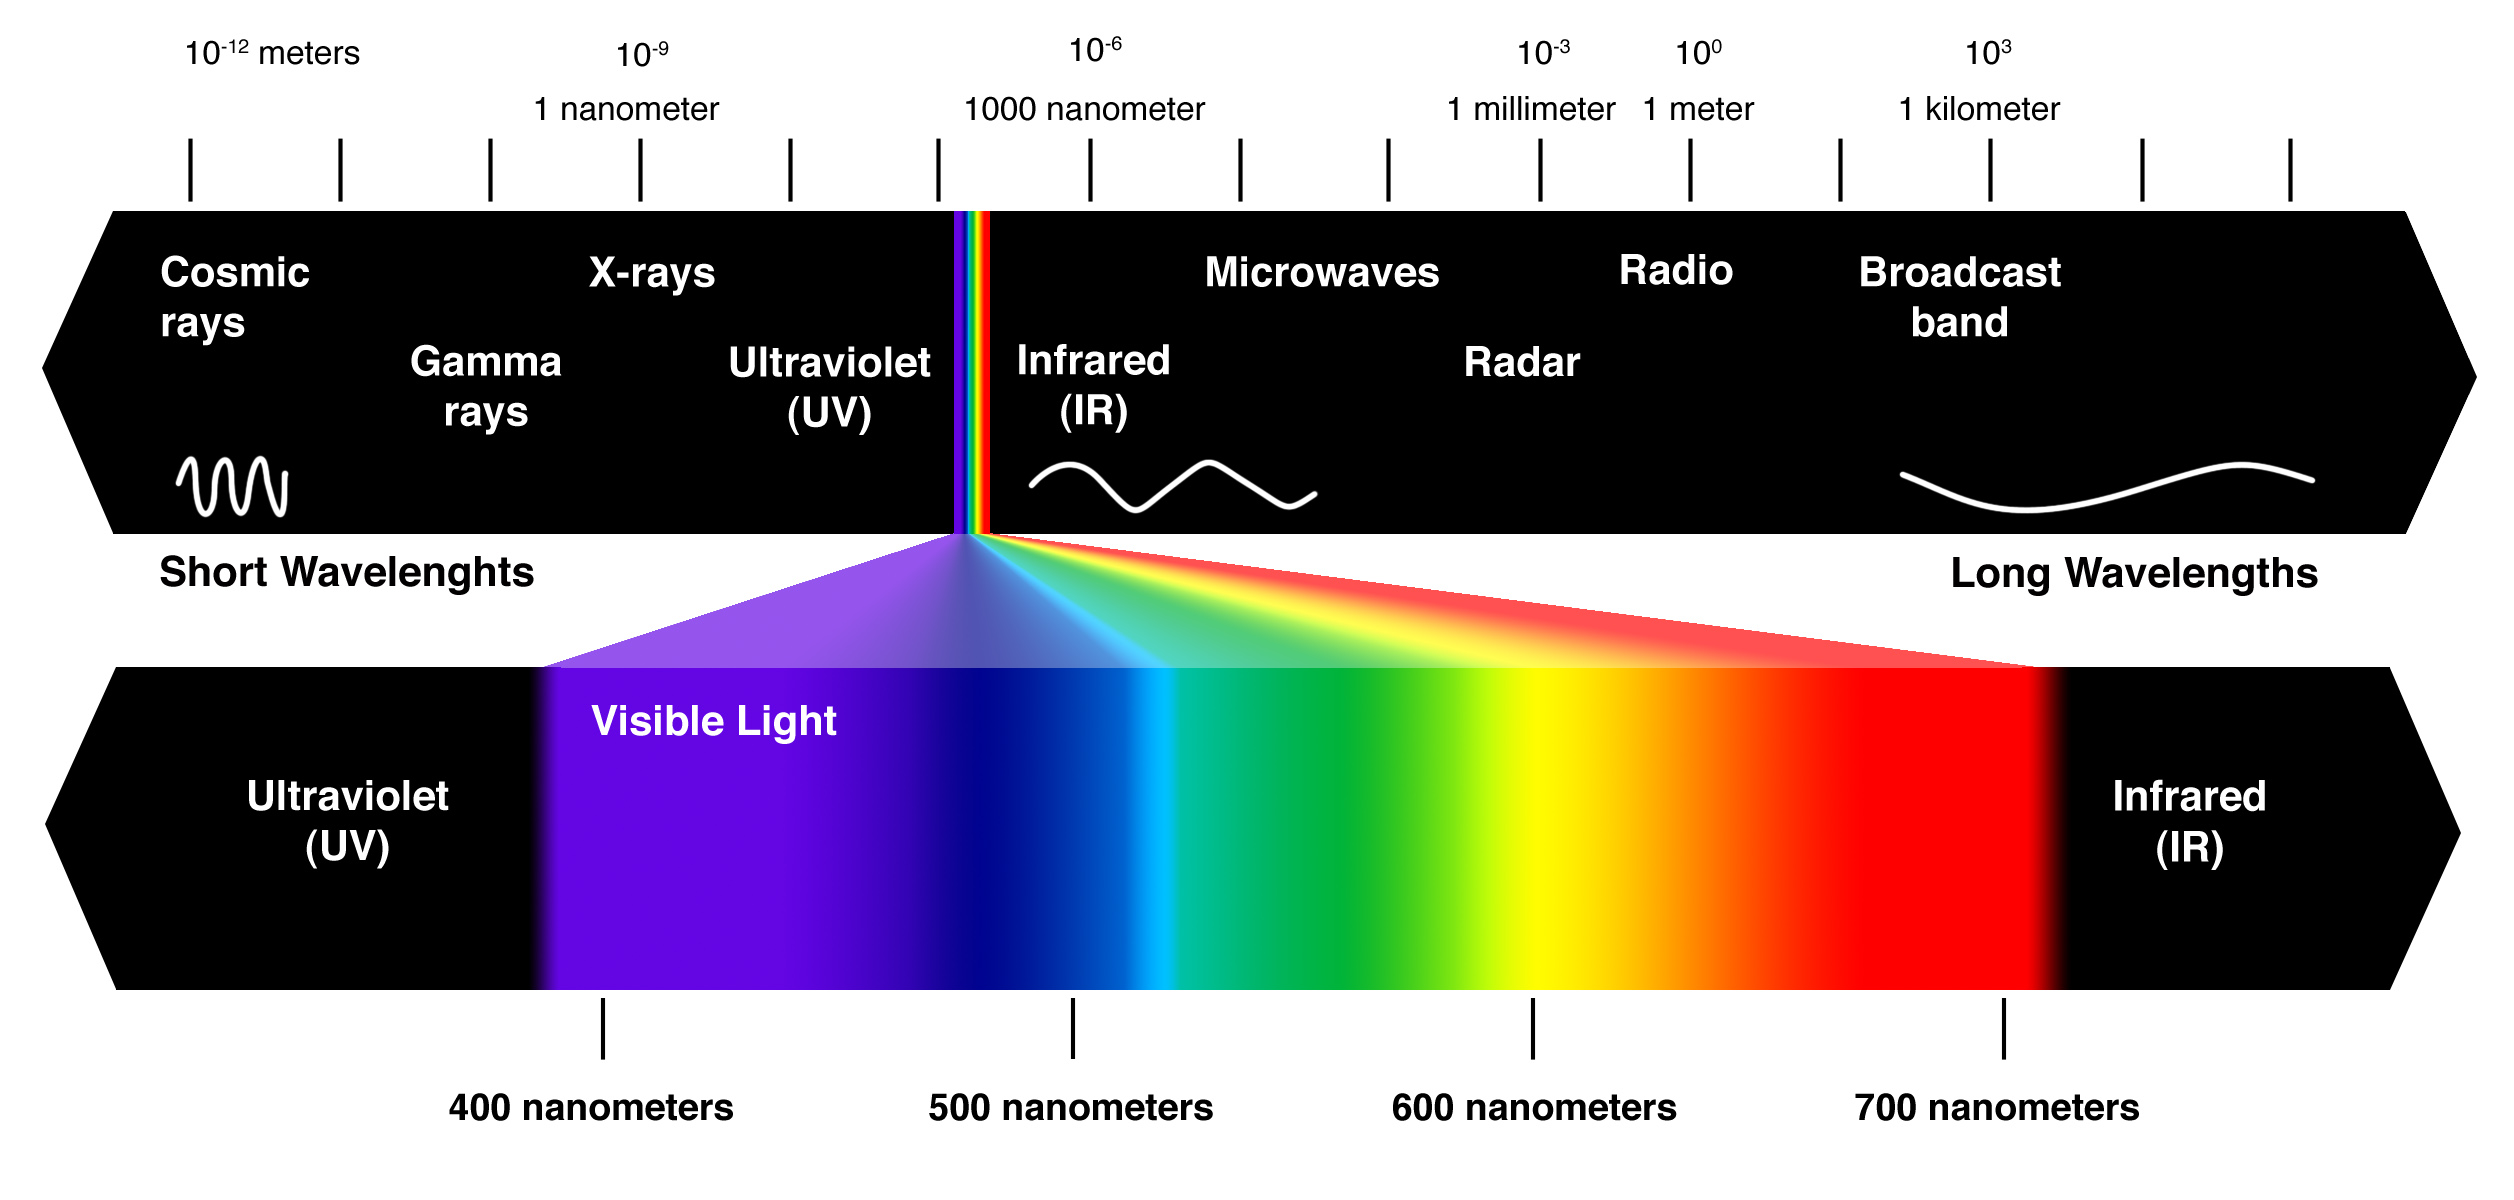
\includegraphics[width=0.65\textwidth]{lqfJrASnQ0GrsLviicAQ_Visible-spectrum.jpeg}
	\caption{Composition of the spectrum of electromagnetic waves}
	\label{fig:spectrum}
\end{figure}